
 \documentclass[12pt]{article}
\usepackage{graphicx}
\usepackage{booktabs}
 \usepackage{makecell}
 \usepackage{float}
 \newcommand{\diff}{\,\mathrm{d}}
\usepackage[margin=1in]{geometry}
\usepackage{fancyhdr}
\pagestyle{fancy}
\usepackage{extarrows}
\usepackage{breqn}

\newcommand{\N}{\mathbb{N}}
\newcommand{\Z}{\mathbb{Z}}
\newcommand{\trans}{^{\mathrm T}}
\usepackage{amssymb}
\usepackage[table]{xcolor}
\usepackage{bm}
\usepackage{array}
\usepackage{mathtools}
\usepackage[english]{babel}
\usepackage{natbib}
\usepackage{url}
\usepackage[utf8x]{inputenc}
\usepackage{amsmath}
\usepackage{graphicx}
\graphicspath{{images/}}
\usepackage{parskip}
\usepackage{fancyhdr}
\usepackage{vmargin}
\usepackage[font={bf, footnotesize}, textfont=md]{caption}
\usepackage{amsmath,amsthm,amssymb}


\newenvironment{theorem}[2][Theorem]{\begin{trivlist}
\item[\hskip \labelsep {\bfseries #1}\hskip \labelsep {\bfseries #2.}]}{\end{trivlist}}
\newenvironment{lemma}[2][Lemma]{\begin{trivlist}
\item[\hskip \labelsep {\bfseries #1}\hskip \labelsep {\bfseries #2.}]}{\end{trivlist}}
\newenvironment{exercise}[2][Exercise]{\begin{trivlist}
\item[\hskip \labelsep {\bfseries #1}\hskip \labelsep {\bfseries #2.}]}{\end{trivlist}}
\newenvironment{reflection}[2][Reflection]{\begin{trivlist}
\item[\hskip \labelsep {\bfseries #1}\hskip \labelsep {\bfseries #2.}]}{\end{trivlist}}
\newenvironment{proposition}[2][Proposition]{\begin{trivlist}
\item[\hskip \labelsep {\bfseries #1}\hskip \labelsep {\bfseries #2.}]}{\end{trivlist}}
\newenvironment{corollary}[2][Corollary]{\begin{trivlist}
\item[\hskip \labelsep {\bfseries #1}\hskip \labelsep {\bfseries #2.}]}{\end{trivlist}}
\DeclareMathOperator{\tr}{tr}
\DeclareMathOperator{\rank}{rank}
\DeclareMathOperator{\Span}{span}
\DeclareMathOperator{\row}{row}
\DeclareMathOperator{\col}{col}
\DeclareMathOperator{\range}{range}
\DeclarePairedDelimiterX{\inp}[2]{\langle}{\rangle}{#1, #2}
\DeclareMathOperator{\Proj}{Proj}
\DeclareMathOperator{\trace}{trace}
\newcommand{\Her}{^{\mathrm H}}
\DeclareMathOperator{\diag}{diag}
\makeatletter 
    \newcommand\fcaption{\def\@captype{table}\caption}
\makeatother
\setmarginsrb{3 cm}{2.5 cm}{3 cm}{2.5 cm}{1 cm}{1.5 cm}{1 cm}{1.5 cm}
\setlength\parindent{1em}

\title{Short Report: Large Amplitude Pendulum}                             % Title
\author{Chen Ang}                               % Author
\date{\today}                                           % Date

\makeatletter
\let\thetitle\@title
\let\theauthor\@author
\let\thedate\@date
\makeatother

\pagestyle{fancy}
\fancyhf{}
\rhead{\theauthor}
\lhead{\thetitle}
\cfoot{\thepage}

\begin{document}

%%%%%%%%%%%%%%%%%%%%%%%%%%%%%%%%%%%%%%%%%%%%%%%%%%%%%%%%%%%%%%%%%%%%%%%%%%%%%%%%%%%%%%%%%

\begin{titlepage}
    \centering
    \vspace*{0.5 cm}
    
\includegraphics[scale = 0.75,width=6cm]{CUHK}\\[1.0 cm]   % University Logo
    \textsc{\large The Chinese University of Hong Kong, Shenzhen}\\[2.0 cm]   % University Name
    \textsc{\Large PHY 1002}\\[0.5 cm]               % Course Code
    \textsc{\large Physics Laboratory}\\[0.5 cm]               % Course Name
    \rule{\linewidth}{0.2 mm} \\[0.4 cm]
    { \huge \bfseries \thetitle}\\
    \rule{\linewidth}{0.2 mm} \\[1.5 cm]
    
    \begin{minipage}{0.4\textwidth}
        \begin{flushleft} \large
            \emph{Author:}\\
            \theauthor
            \\
            \emph{Group Number:} \\
            Group 1
            \end{flushleft}
            \end{minipage}~
            \begin{minipage}{0.4\textwidth}
            \begin{flushright} \large
            \emph{Student Number:} \\
            118010009                                   % Your Student Number
            \\
            \emph{Experiment Date:}\\
            September 27, 2019
        \end{flushright}
    \end{minipage}\\[2 cm]
    
    {\large \thedate}\\[2 cm]
 
    \vfill
    
\end{titlepage}

%%%%%%%%%%%%%%%%%%%%%%%%%%%%%%%%%%%%%%%%%%%%%%%%%%%%%%%%%%%%%%%%%%%%%%%%%%%%%%%%%%%%%%%%%
%%%%%%%%%%%%%%%%%%%%%%%%%%%%%%%%%%%%%%%%%%%%%%%%%%%%%%%%%%%%%%%%%%%%%%%%%%%%%%%%%%%%%%%%%

\tableofcontents
\pagebreak


%%%%%%%%%%%%%%%%%%%%%%%%%%%%%%%%%%%%%%%%%%%%%%%%%%%%%%%%%%%%%%%%%%%%%%%%%%%%%%%%%%%%%%%%%

\rmfamily
\section{Small Amplitude Pendulum}
\subsection{Data Analysis}
\begin{figure}[H]
	\centering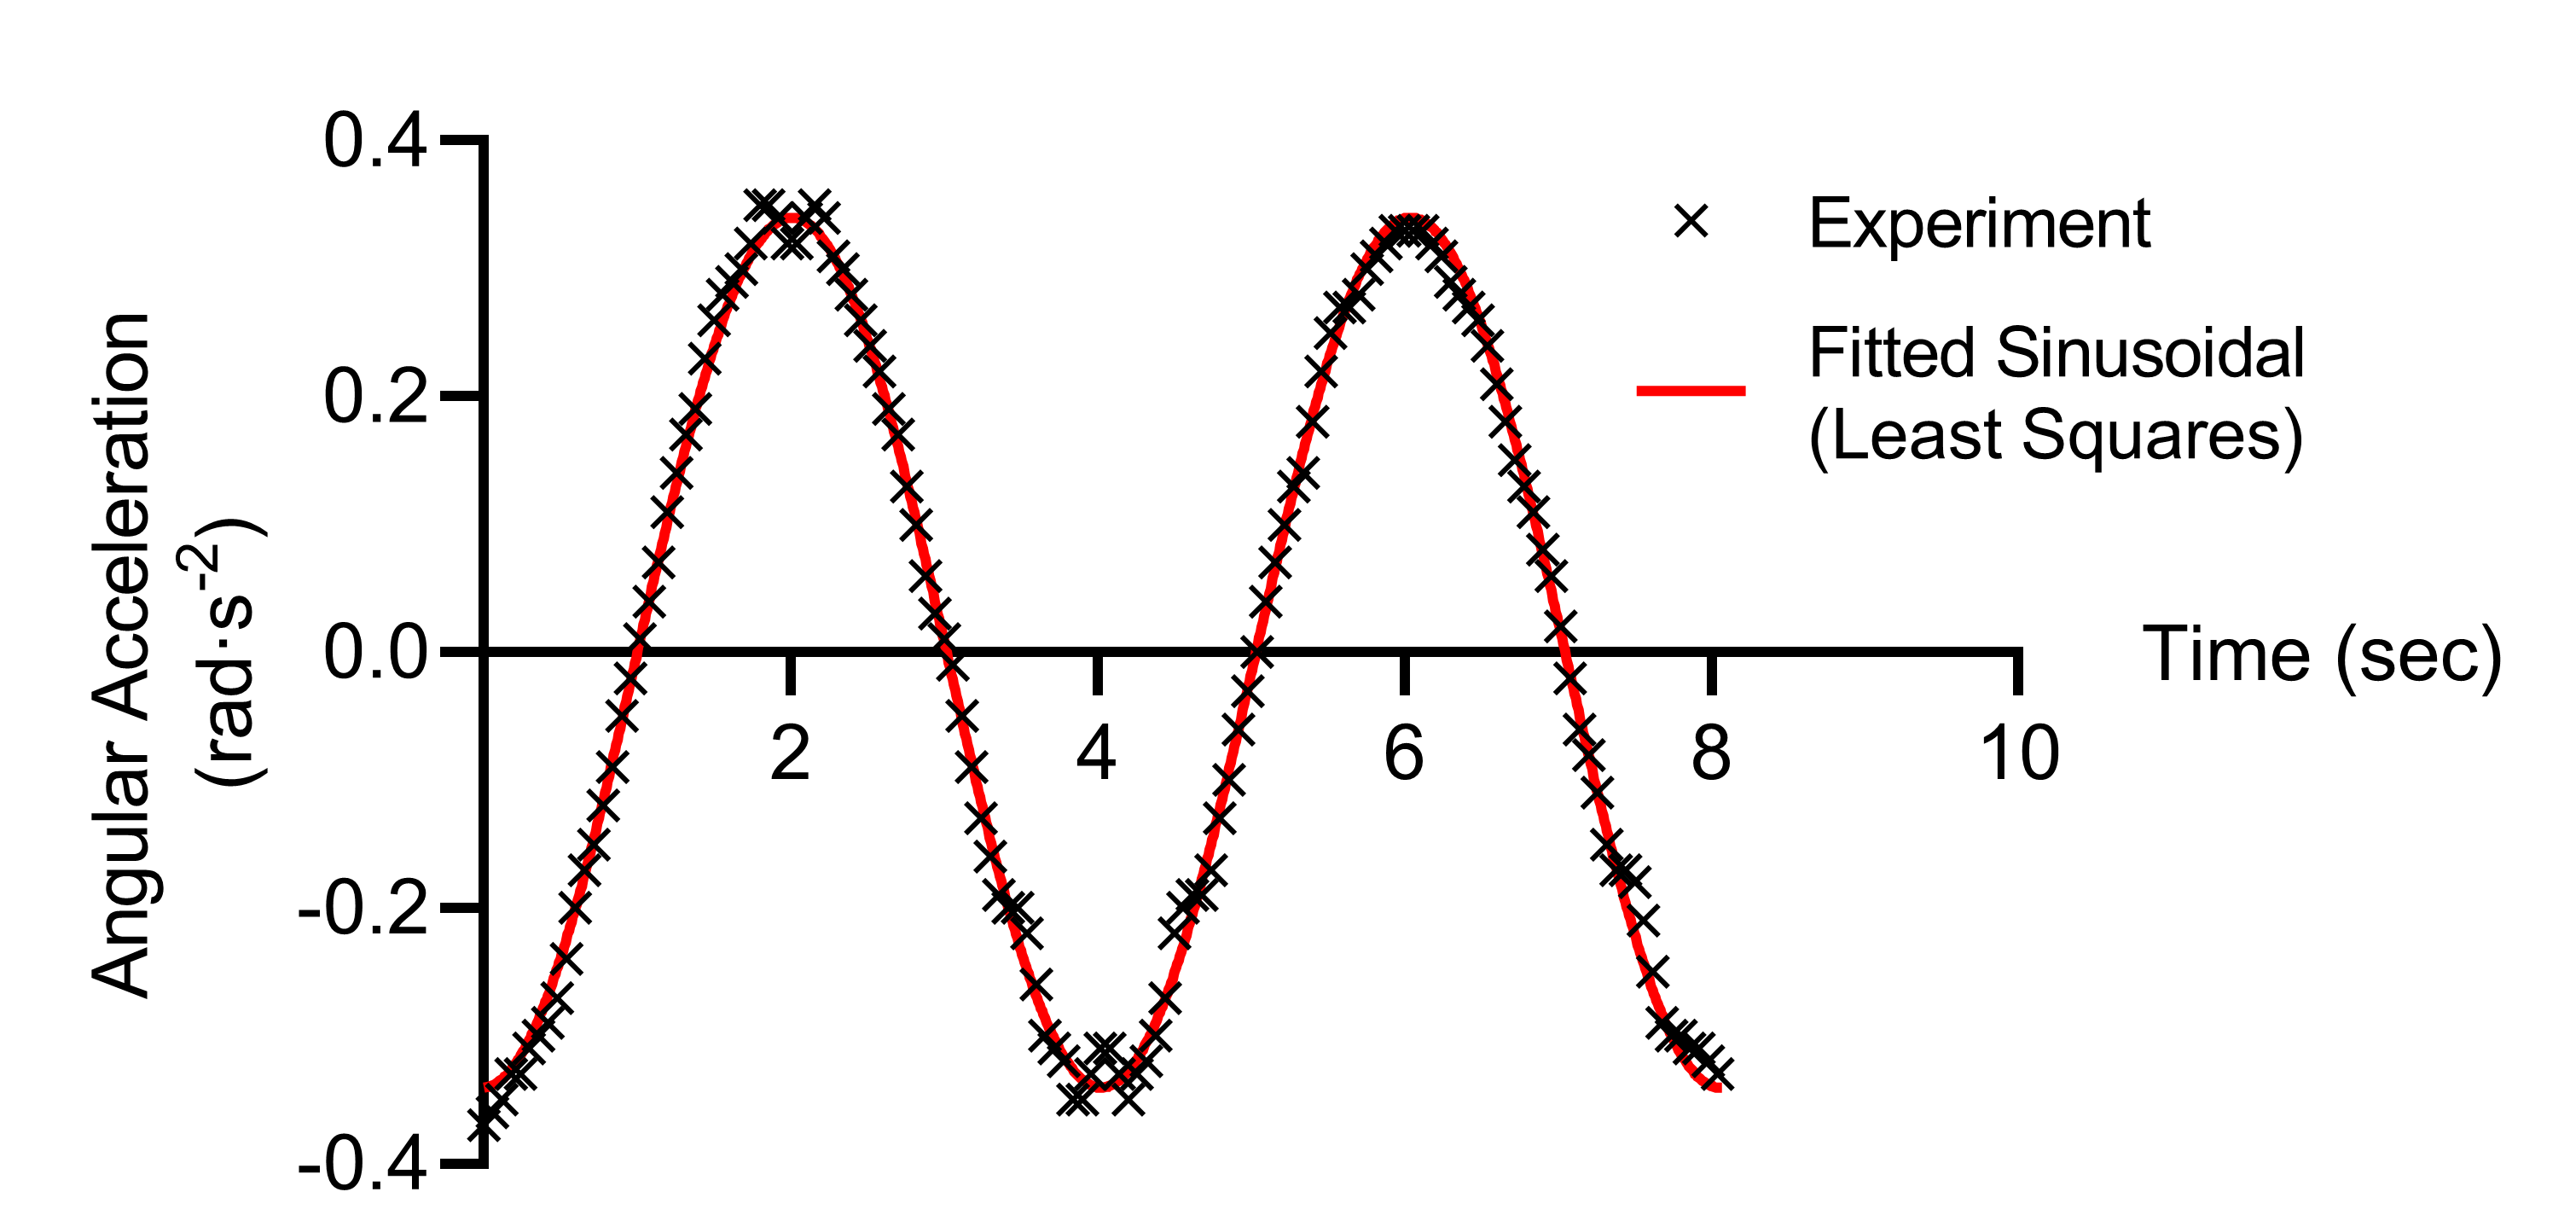
\includegraphics[width=10cm]{at}
	\caption{$\alpha$-$t$ graph at a small amplitude ($<0.35$ rad)}
	\label{$Frequency-Intensity$ Graph for $70$cm tube}
\end{figure}
The experimental data is well fitted ($R^2=0.9966$) with the sinusoidal (Amp $= 0.3401$ rad·s$^{-2}$;  $T=4.03 \text{ sec}$). We obtain the following from experiment:
$$
2T_0=8.08\pm 0.02 \text{ sec};\ 
\theta_0=0.141\pm 0.001 \text{ rad}
.
$$
The theoretical values are
$$
\begin{aligned}
T_0&=4.04\pm 0.01\text{ sec};\\
\text{Amp}_{\text{theo}}&=
A^2\theta_0\\&=\frac{4\pi^2\theta_0}{T_0^2}\\&=0.3410\pm0.0029\text{ rad·s}^{-2}.
\end{aligned}
$$
A nice agreement can be seen from the following table
$$
\begin{tabular}{|c|c|c|}
	\hline 
	& 预测  & Experiment (Curve Fitting) \\ 
	\hline 
Amplitude (rad·s$^{-2}$)	& 4.04 $\pm$ 0.01  & 4.03 \\ 
	\hline
Period (sec)	& 0.3410 $\pm$ 0.0029 & 0.3401 \\ 
	\hline 
\end{tabular} 
$$
The minimal discrepancy confirms the validity of the theory.

\subsection{Question}
\begin{enumerate}
	\item \emph{Why is the minus sign in the expression of angular acceleration?}
	
	\textbf{Answer: }The angular acceleration is in the same direction as the restoring torque, which, is always in the opposite direction of the angular displacement.
\end{enumerate}


\section{Large Amplitude Pendulum}
\subsection{Data Analysis}
\begin{figure}[H]
	\centering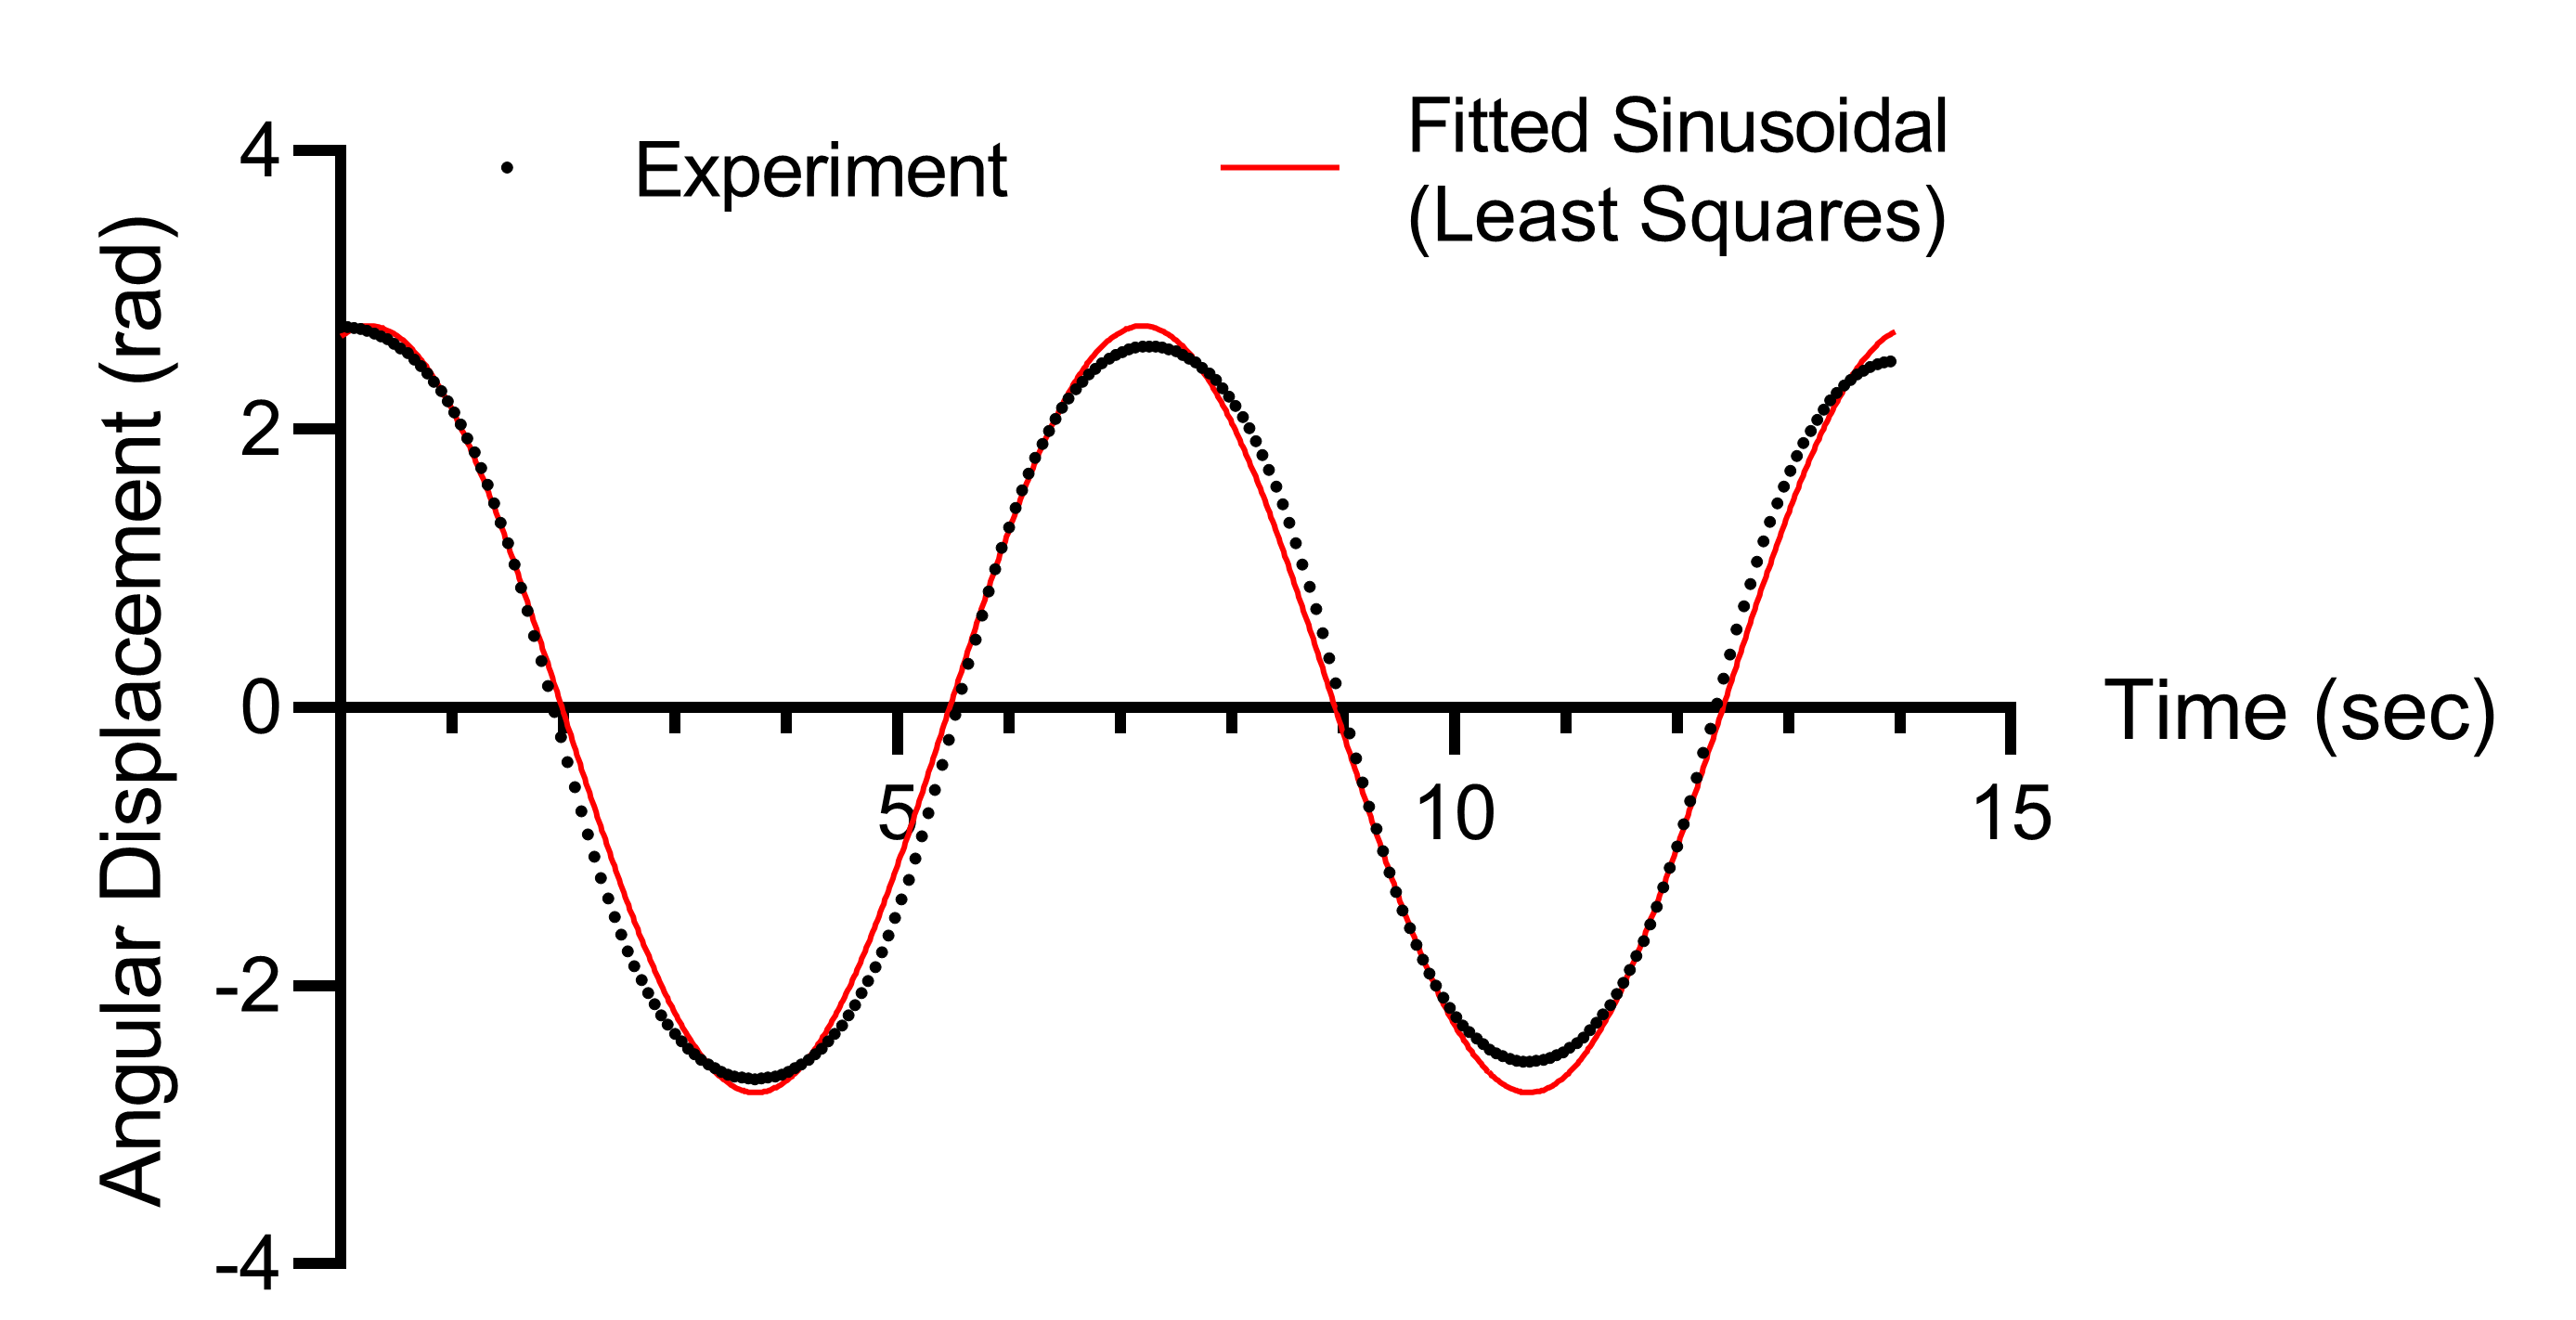
\includegraphics[width=10cm]{lg}
	\caption{$\theta$-$t$ graph at a large amplitude ($\approx3$ rad)}
\end{figure}
At a large amplitude, the shape of the experimental data becomes more deviated from the fitted sinusoidal ($R^2=0.9925$). This suggest that the small-angle approximation fails to depict an accurate picture as $\theta_0$ approaches $\pi$ rad.

\subsection{Questions}
\begin{enumerate}
	\item \emph{Is this curve sinusoidal?}
	
	\textbf{Answer: }No, as noticable deviation is present from the fitted sinusoidal in Figure 2.
$$$$
	\item \emph{What is the displacement/acceleration corresponding to the turning point, when the speed is zero or maximum?}
	
	\textbf{Answer: }The displacement and acceleration are both zero when the velocity reaches maximum (in magnitude). When the velocity is zero, the displacement reaches maximum (in magnitude) while the acceleration is at a local minimum (in magnitude) (See Figure 3).
	\begin{figure}[H]
		\centering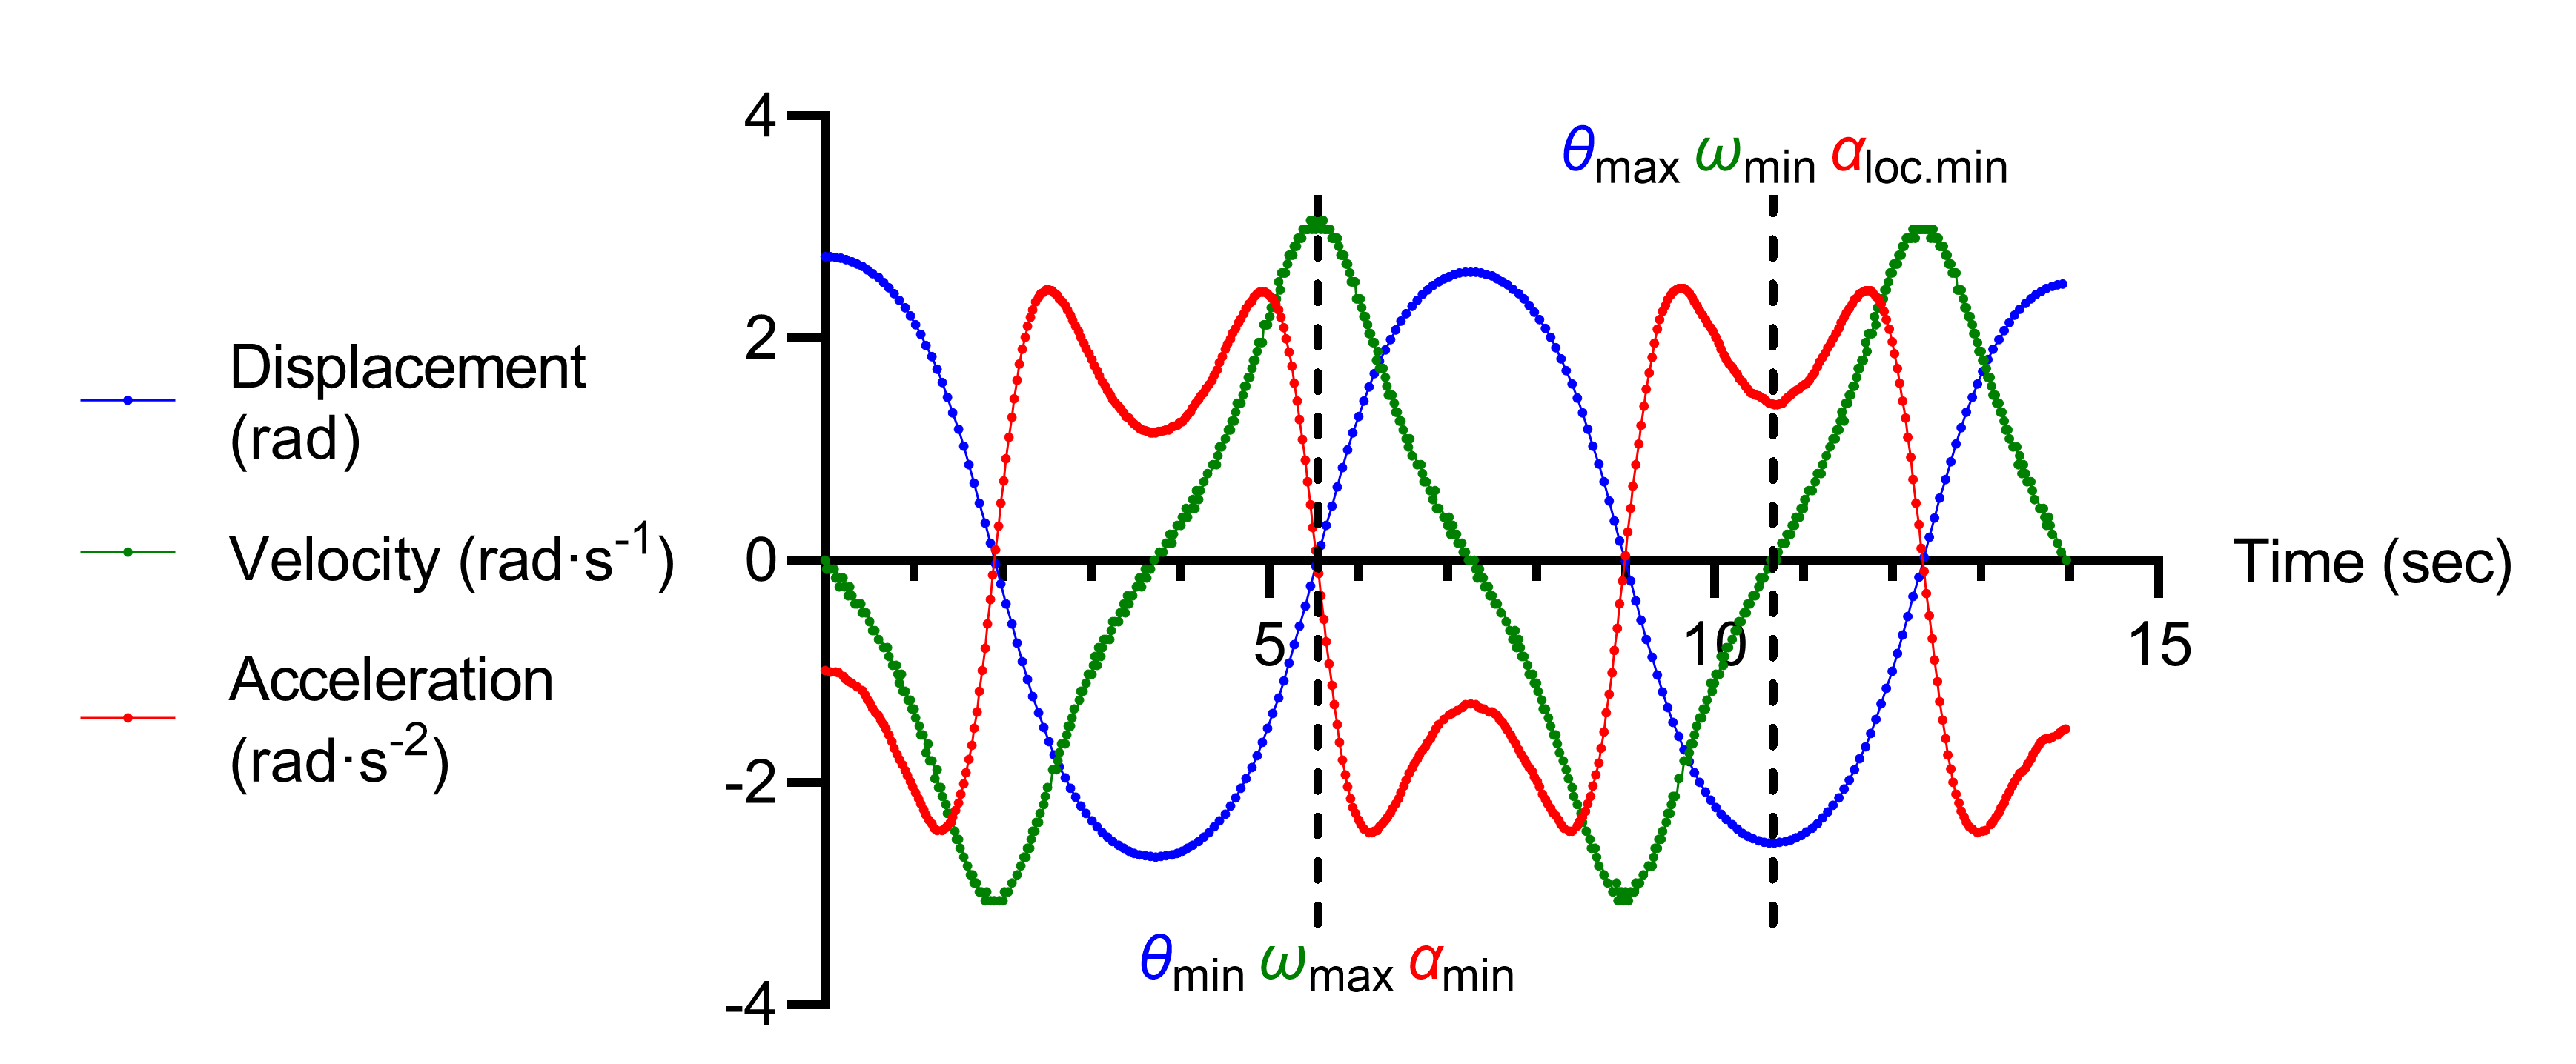
\includegraphics[width=13cm]{lgg}
		\caption{$\theta$-$\omega$-$\alpha$-$t$ graph at a large amplitude ($\approx 3$ rad)}
		\label{$Frequency-Intensity$ Graph for $70$cm tube}
	\end{figure}
\end{enumerate}



\end{document}
